\chapter{Methodology}\label{cha:methodology}

The proposed self-healing security framework operates across two distinct environments: a lightweight edge layer for real-time anomaly detection and risk scoring, and a cognitive cloud layer for threat classification, XAI feature extraction, and multi-agent remediation.

\begin{figure}[htbp]
	\begin{center}
		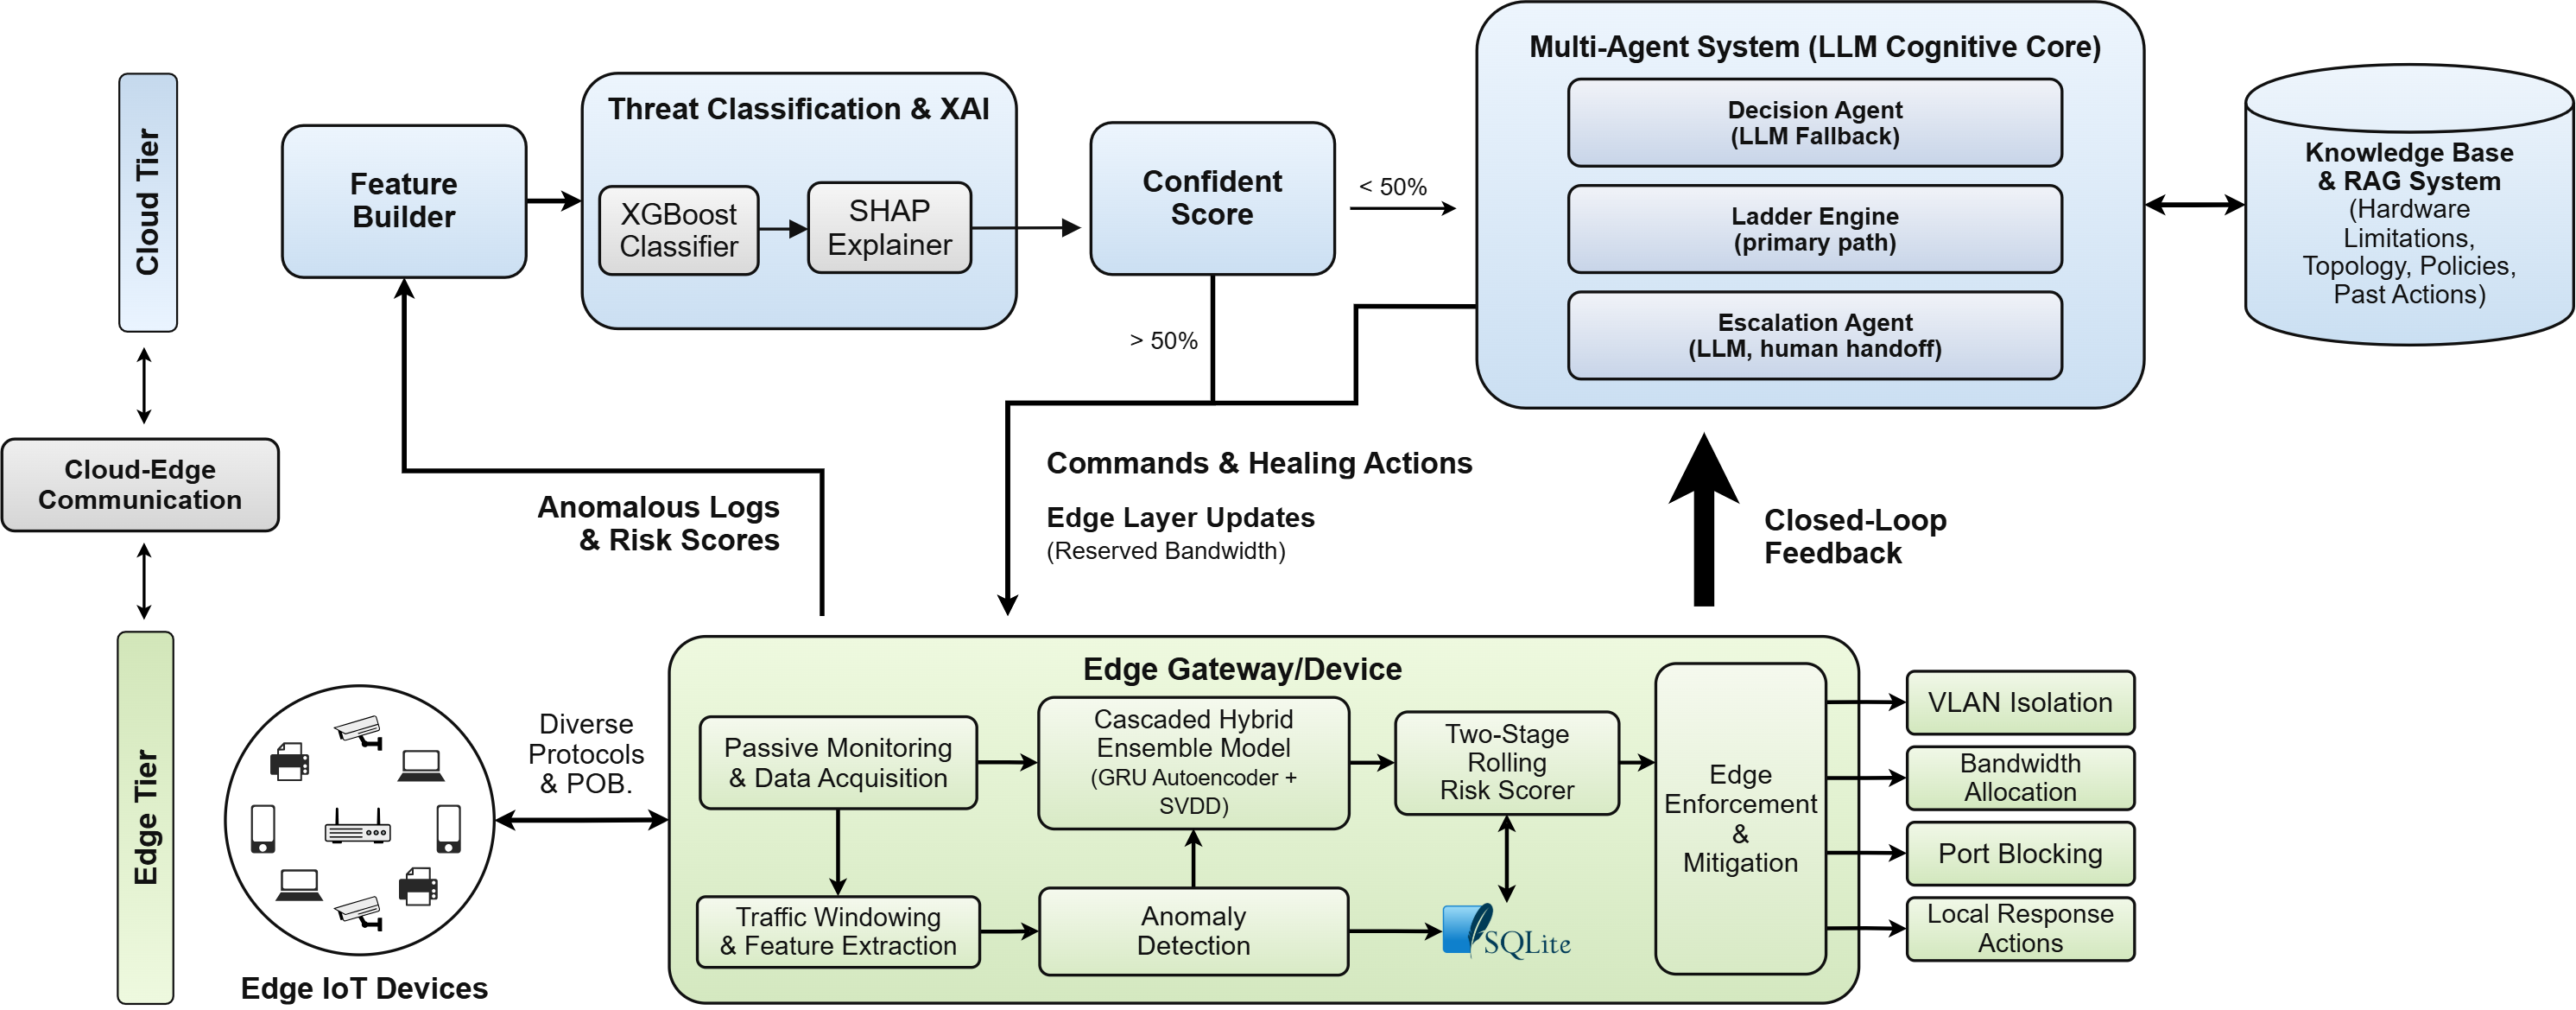
\includegraphics[width=5in]{Images/system_architecture.png}
	\end{center}
	\caption{High-level system architecture. The edge tier runs its own GRU+Deep SVDD anomaly ensemble and rolling risk score entirely locally (dashed box); as discussed in Section \ref{sec:cloud_classification}, this score is not currently transmitted to the cloud, which classifies every raw windowed telemetry submission independently. In the cloud tier, a deterministic Ladder Engine is the primary healing-decision path; the Decision and Escalation Agents are LLM-backed fallbacks consulted only when the ladder cannot resolve an incident on its own (Section \ref{sec:multi_agent}), and the Dashboard Reporting Agent runs in parallel on every classified window.}
	\label{fig:architecture}
\end{figure}

\section{Edge Layer: Traffic Monitoring and Representation}

At the edge layer, passive network monitoring is employed to capture IoT traffic without introducing latency into device operations. As shown in Figure \ref{fig:architecture}, this responsibility is split across two modules within the Edge Gateway/Device: \textbf{Passive Monitoring \& Data Acquisition}, which observes traffic from the attached IoT device population without inserting itself into the data path, and \textbf{Traffic Windowing \& Feature Extraction}, which aggregates the captured traffic into time-based windows and derives the statistical and behavioral descriptors used by the detection ensemble.

Passive monitoring is implemented through observation of traffic that is already traversing the gateway-for example, via port mirroring on a managed switch or a network tap positioned ahead of the gateway's forwarding path-so that the acquisition step itself adds no additional hops, and therefore no additional latency, to the traffic it observes. This is a deliberate design constraint rather than an implementation detail: Chapter \ref{cha:introduction} establishes that the endpoint population this framework protects cannot tolerate an inline security appliance that introduces its own processing delay, since several of the attack patterns motivating this work conclude within seconds to a few minutes, and any latency contributed by the detection pipeline itself would eat directly into an already narrow window for response.

From the raw captured traffic, the Traffic Windowing \& Feature Extraction module aggregates packets into fixed-length time windows per device and computes a fixed set of 36 statistical and behavioral descriptors for each window, listed in full in Table \ref{tb:feature_register}. These fall into two families: five \texttt{log\_*} features summarising the application- or message-layer traffic observed in the window (message counts, inter-message interval statistics, and the range and type diversity of the data values carried), and 31 \texttt{network\_*} features summarising the packet- and connection-layer traffic (header length, IP length and flags, TCP maximum-segment-size, TCP control-flag counts, inter-packet timing, IP time-to-live, and the cardinality of distinct source/destination IP addresses, MAC addresses, ports, and protocols observed). This split reflects the two levels at which the edge gateway can observe a constrained IoT device: what it is saying, at the level of the messages an application-layer protocol exchanges, and how it is saying it, at the level of the underlying packet stream-consistent with the general family of flow-level statistical features used throughout the network-intrusion-detection literature reviewed in Chapter \ref{cha:literature_review}, but fixed here to the specific 36-feature schema the edge-layer models were trained and evaluated against. The resulting per-window feature vector is normalized using a pre-fitted \texttt{MinMaxScaler}, which rescales each feature to the $[0,1]$ range using minimum and maximum values fitted on a benign-traffic calibration set, so that features with different natural scales (e.g., a byte count in the thousands versus a protocol-distribution ratio between 0 and 1) contribute comparably to the downstream model rather than being dominated by whichever feature happens to have the largest raw magnitude. These normalized point features, denoted $x_{scaled}$, serve as one of the two inputs to the anomaly detection ensemble described in Section \ref{sec:hybrid_ensemble}; the other being the sliding window of recent frames consumed by the temporal model.
{\small
\renewcommand{\arraystretch}{1.15}
\begin{longtable}{|>{\centering\arraybackslash}p{0.05\textwidth}|>{\raggedright\arraybackslash}p{0.34\textwidth}|>{\raggedright\arraybackslash}p{0.49\textwidth}|}
\caption{Complete edge-layer feature register: the 36 statistical and behavioral descriptors computed per traffic window and consumed by the GRU + Deep SVDD ensemble.}
\label{tb:feature_register}\\
\hline
\textbf{\#} & \textbf{Feature name} & \textbf{Description} \\
\hline
\endfirsthead
\multicolumn{3}{|c|}{\tablename\ \thetable{} -- continued from previous page}\\
\hline
\textbf{\#} & \textbf{Feature name} & \textbf{Description} \\
\hline
\endhead
\multicolumn{3}{|r|}{\textit{Continued on next page}}\\
\hline
\endfoot
\endlastfoot
0 & \path{log_data-ranges_avg} & Average range spanned by data values carried in the window's application/log-level messages. \\ \hline
1 & \path{log_data-ranges_std_deviation} & Standard deviation of the same data-range measure. \\ \hline
2 & \path{log_data-types} & Diversity of data types observed across the window's log-level messages (small integer-coded categorical). \\ \hline
3 & \path{log_interval-messages} & Inter-message interval statistic at the application/log-message level. \\ \hline
4 & \path{log_messages_count} & Count of application/log-level messages observed in the window. \\ \hline
5 & \path{network_header-length_avg} & Average packet header length. \\ \hline
6 & \path{network_header-length_std_deviation} & Standard deviation of packet header length. \\ \hline
7 & \path{network_interval-packets} & Inter-packet interval statistic. \\ \hline
8 & \path{network_ip-flags_avg} & Average value of the IP header flags field. \\ \hline
9 & \path{network_ip-flags_min} & Minimum value of the IP header flags field. \\ \hline
10 & \path{network_ip-length_avg} & Average IP total-length field value. \\ \hline
11 & \path{network_ip-length_max} & Maximum IP total-length field value. \\ \hline
12 & \path{network_ip-length_min} & Minimum IP total-length field value. \\ \hline
13 & \path{network_ips_all} & Cardinality/encoding of all distinct IP addresses (source and destination) observed. \\ \hline
14 & \path{network_ips_all_count} & Count of distinct IP addresses observed. \\ \hline
15 & \path{network_ips_dst} & Cardinality/encoding of distinct destination IP addresses observed. \\ \hline
16 & \path{network_macs_all} & Cardinality/encoding of distinct MAC addresses observed. \\ \hline
17 & \path{network_mss_avg} & Average TCP Maximum Segment Size. \\ \hline
18 & \path{network_mss_std_deviation} & Standard deviation of TCP Maximum Segment Size. \\ \hline
19 & \path{network_packet-size_avg} & Average packet size. \\ \hline
20 & \path{network_packet-size_min} & Minimum packet size. \\ \hline
21 & \path{network_packets_all_count} & Total packet count in the window. \\ \hline
22 & \path{network_ports_all} & Cardinality/encoding of distinct ports observed. \\ \hline
23 & \path{network_ports_all_count} & Count of distinct ports observed. \\ \hline
24 & \path{network_protocols_all} & Cardinality/encoding of distinct protocols observed. \\ \hline
25 & \path{network_protocols_all_count} & Count of distinct protocols observed. \\ \hline
26 & \path{network_protocols_dst} & Cardinality/encoding of distinct destination-side protocols. \\ \hline
27 & \path{network_protocols_src} & Cardinality/encoding of distinct source-side protocols. \\ \hline
28 & \path{network_tcp-flags-fin_count} & Count of TCP FIN flags observed. \\ \hline
29 & \path{network_tcp-flags-rst_count} & Count of TCP RST flags observed. \\ \hline
30 & \path{network_tcp-flags-syn_count} & Count of TCP SYN flags observed. \\ \hline
31 & \path{network_time-delta_avg} & Average inter-arrival time delta between packets. \\ \hline
32 & \path{network_time-delta_max} & Maximum inter-arrival time delta. \\ \hline
33 & \path{network_time-delta_min} & Minimum inter-arrival time delta. \\ \hline
34 & \path{network_time-delta_std_deviation} & Standard deviation of inter-arrival time delta. \\ \hline
35 & \path{network_ttl_avg} & Average IP time-to-live value. \\ \hline
\end{longtable}
}

\section{Cascaded Hybrid (Stacked) Ensemble Model}\label{sec:hybrid_ensemble}

To robustly identify anomalous behavior without requiring labeled attack data during training, the edge layer deploys a one-class cascaded hybrid ensemble, shown as the \textbf{Cascaded Hybrid Ensemble Model (GRU Autoencoder + Deep SVDD)} block in Figure \ref{fig:architecture}. This architecture pairs a deep temporal model with a deep one-class boundary method, leveraging the strengths of both: the GRU autoencoder captures how a device's traffic evolves over a short recent history, while Deep Support Vector Data Description (Deep SVDD) provides a compact, unsupervised description of what a benign combination of temporal and point-in-time features looks like, against which any new observation can be scored. Figure \ref{fig:hybrid_ensemble} expands this block into its constituent pipeline, showing how the GRU's temporal embedding and the current timestep's scaled point features are concatenated before being scored by the Deep SVDD boundary; the three numbered steps below correspond directly to the stages shown in that diagram.

\begin{enumerate}
	\item \textbf{Temporal Feature Extraction:} A single-layer Gated Recurrent Unit (GRU) autoencoder \cite{Cho2014} with a hidden dimension of 64 processes a sliding window of recent frames (size 8). The GRU is a simplified recurrent architecture that merges the input and forget gates of a Long Short-Term Memory (LSTM) cell into a single update gate and removes the separate cell state, which reduces the number of trainable parameters and the per-step computation relative to an LSTM while retaining the ability to model sequential dependencies in the traffic-the property this project relies on to build a temporal fingerprint of device behavior. The GRU is trained as an autoencoder, i.e., it is optimized to reconstruct its own input window rather than to predict a label, so that its reconstruction error is large precisely when the input window departs from the sequential patterns seen in benign training traffic. The GRU is optimized using the RMSprop algorithm \cite{Tieleman2012} ($\alpha=0.99$, learning rate $0.002$). RMSprop is specifically selected over Adam because its moving average of squared gradients better stabilizes training against the noisy, non-stationary reconstruction loss typical of IoT traffic. The last hidden state of the GRU, $h_n[-1]$, serves as a 64-dimensional temporal embedding representing sequential device behavior.

	\item \textbf{Feature Fusion and One-Class Boundary Estimation:} The temporal embedding is concatenated with the current timestep's MinMax-scaled point features to create a fused feature vector, $v_{fused} = h_n[-1] \oplus x_{scaled}$. This fused vector is the input to a Deep Support Vector Data Description (Deep SVDD) model \cite{Ruff2018}, trained entirely on benign traffic. Deep SVDD extends the classical, kernel-based SVDD of Tax and Duin \cite{Tax2004} by replacing the fixed kernel-induced feature map with a neural network $\phi(\cdot\,; W)$ whose weights $W$ are learned jointly with the one-class objective, rather than fixed in advance or selected from a small family of kernel functions. In the one-class variant used here-appropriate because the training set is (assumed) entirely benign, so no soft boundary or outlier-tolerance slack term is required-the network is trained to map every benign training vector as close as possible to a fixed centre $c$ in the output space:
	\begin{equation}
	\min_{W} \; \frac{1}{n} \sum_{i=1}^{n} \lVert \phi(v_i; W) - c \rVert^2 \; + \; \frac{\lambda}{2} \sum_{l} \lVert W_l \rVert_F^2,
	\label{e:svdd_primal}
	\end{equation}
	where $n$ is the number of benign training vectors, $c$ is fixed in advance (for example, as the mean of an initial forward pass over the training set, following \cite{Ruff2018}) rather than optimised jointly, $\lambda$ is a weight-decay regularisation coefficient applied per layer $l$, and the network $\phi(\cdot\,;W)$ is constructed without bias terms and without bounded activation functions in its final layers, an architectural constraint Ruff et al. show is necessary to prevent the trivial ``hypersphere collapse'' solution in which the network learns to map every input to $c$ regardless of its content \cite{Ruff2018}. Minimising Equation \ref{e:svdd_primal} concentrates the benign training population as tightly as possible around $c$ in the learned output space, so that a genuinely benign vector observed at inference time is expected to land close to $c$, while a vector whose fused temporal-and-point-feature profile differs materially from benign behaviour is expected to land further away. This is the property that makes the resulting distance a usable one-class anomaly score, and is exactly analogous to the volume-minimisation intuition of classical SVDD's hypersphere, but achieved through a learned representation rather than a fixed kernel.

	\item \textbf{Inference:} At runtime, a new fused feature vector $v$ is scored by its squared distance from the learned centre,
	\begin{equation}
	d(v) = \lVert \phi(v; W) - c \rVert^2,
	\label{e:svdd_score}
	\end{equation}
	which is small when $v$ resembles the benign training population and large when it does not. This continuous distance score $d(v)$ is compared against an optimal threshold (determined offline via the F1 precision-recall curve on a validation set) to flag the time window as anomalous, corresponding to the \textbf{Anomaly Detection} step in Figure \ref{fig:architecture}.
\end{enumerate}

Deep SVDD is preferred over a purely distance-based or density-based one-class method for this fused vector for two reasons specific to this design. First, because $v_{fused}$ concatenates a 64-dimensional learned temporal embedding with a smaller set of point features, the two halves of the vector have different statistical structure, and a jointly learned neural boundary can adapt to this combined space more flexibly than a boundary defined directly in terms of Euclidean distance to training examples, or than a fixed kernel selected without reference to the specific structure of a GRU-produced embedding. Second, Deep SVDD's boundary is defined purely from benign data and does not require an attack-labeled dataset during training, which matches the practical constraint-already discussed in Chapter \ref{cha:literature_review}-that verified attack traffic for a given IoT deployment is typically far scarcer than benign traffic, and often unavailable altogether prior to deployment. Chapter \ref{cha:results} reports that, on the evaluation data available for this project, a standalone Deep SVDD model performs considerably worse than the fused GRU + Deep SVDD ensemble, which is the empirical justification, alongside the architectural reasoning above, for pairing it with the GRU's temporal embedding rather than deploying it directly on point features alone.

\begin{figure}[htbp]
	\begin{center}
	\resizebox{5in}{!}{%
	\begin{tikzpicture}[
		>=Stealth,
		node distance=1.5cm and 2cm,
		box/.style={draw, rectangle, rounded corners, minimum width=3cm, minimum height=1cm, align=center, fill=blue!5},
		model/.style={draw, rectangle, rounded corners, minimum width=3cm, minimum height=1cm, align=center, fill=purple!5, thick},
		fusion/.style={draw, circle, minimum size=1.5cm, align=center, fill=green!5, thick},
		decision/.style={draw, diamond, aspect=2, minimum width=2.5cm, minimum height=1cm, align=center, fill=orange!5}
	]

	% Nodes
	\node[box] (input) {Raw IoT Traffic Features};
	\node[box, below=1cm of input] (scaler) {MinMaxScaler};

	\node[model, below left=1.5cm and -0.5cm of scaler] (gru) {GRU Autoencoder \\ (hidden\_dim=64)};
	\node[box, below=1cm of gru] (embedding) {Temporal Embedding \\ ($h_n[-1]$)};

	\node[box, below right=1.5cm and -0.5cm of scaler] (point) {Scaled Point Features \\ ($x_{scaled}$)};

	\node[fusion, below right=0.5cm and 1cm of embedding] (concat) {Concat \\ ($\oplus$)};

	\node[model, below=1cm of concat] (svdd) {Deep SVDD \\ (neural network)};
	\node[box, below=1cm of svdd] (score) {Deep SVDD Distance Score \\ ($d(v)$)};

	\node[decision, below=1cm of score] (threshold) {$>$ Threshold?};

	\node[box, fill=red!10, below left=1cm and -0.5cm of threshold] (anomaly) {Anomaly (True)};
	\node[box, fill=green!10, below right=1cm and -0.5cm of threshold] (benign) {Benign (False)};

	% Arrows
	\draw[->, thick] (input) -- (scaler);

	\draw[->, thick] (scaler) -| node[above left, xshift=1cm] {Sliding Window ($t-8$ to $t$)} (gru);
	\draw[->, thick] (scaler) -| node[above right, xshift=-1cm] {Current Timestep ($t$)} (point);

	\draw[->, thick] (gru) -- (embedding);

	\draw[->, thick] (embedding) |- (concat);
	\draw[->, thick] (point) |- (concat);

	\draw[->, thick] (concat) -- node[right] {$v_{fused}$} (svdd);
	\draw[->, thick] (svdd) -- (score);
	\draw[->, thick] (score) -- (threshold);

	\draw[->, thick] (threshold) -| node[above left] {Yes} (anomaly);
	\draw[->, thick] (threshold) -| node[above right] {No} (benign);

	\end{tikzpicture}%
	}
	\end{center}
	\caption{Block diagram of the cascaded hybrid ensemble showing the GRU pipeline and feature concatenation with the Deep SVDD one-class boundary.}
	\label{fig:hybrid_ensemble}
\end{figure}

\FloatBarrier
\section{Two-Stage Rolling Risk Scoring Mechanism}

Instead of triggering alerts on isolated anomalies, the edge system calculates a persistent per-device risk score, $R \in [0,1]$, to identify sustained malicious activity. This is the mechanism shown as the \textbf{Two-Stage Rolling Risk Scorer} in Figure \ref{fig:architecture}, positioned between the ensemble model and the Edge Enforcement \& Mitigation module.

\textbf{Stage 1: Ensemble Scoring.} While the Deep SVDD boundary's binary decision (Equation \ref{e:svdd_score} compared against the fitted threshold) controls the discrete anomaly flag logged at the \textbf{Anomaly Detection} step, a combined continuous score is also generated for every window of telemetry, so that the risk scorer has graded evidence to work with rather than a single bit per window. Both the GRU reconstruction Mean Squared Error (MSE) and the Deep SVDD distance score $d(v)$ are independently normalized to $[0,1]$ using the same offline-fitted scaling bounds used elsewhere in the pipeline, yielding $S_{gru}$ and $S_{svdd}$ respectively.

\textbf{Stage 2: Rolling Risk Scorer.} The risk score $R$ is dynamically updated per window based on a weighted accumulation and decay mechanism. If a window is flagged as anomalous, the score is increased by a delta, $\Delta R$, defined as:
\begin{equation}
\Delta R = \frac{1}{2} \left( W_{hit} + W_{gru} \cdot S_{gru} + W_{svdd} \cdot S_{svdd} + B_{repeat} \right)
\label{e:delta_r}
\end{equation}
where $W_{hit} = 0.35$ is a fixed penalty applied to every flagged window regardless of its score, $W_{gru} = 0.45$ weights the GRU's continuous reconstruction-error contribution, and $W_{svdd} = 0.40$ weights the Deep SVDD boundary's continuous distance-score contribution. The term $B_{repeat}$ is a repeat-offender boost (up to $0.20$), scaled by the number of consecutive anomalous windows (capped at 5), so that a device flagged repeatedly in immediate succession accumulates risk faster than one flagged once and then not again. The new risk score is clamped at a maximum of $1.0$:
\begin{equation}
R_{t} = \min(R_{t-1} + \Delta R, 1.0)
\label{e:risk_increase}
\end{equation}

Conversely, if the window is benign, the consecutive anomaly counter resets, and the score decays by a fixed penalty, bottoming out at a baseline default of $0.05$ (rather than $0$, so that a device with any recent history of suspicion does not require a full re-accumulation from a completely clean state after a single benign window):
\begin{equation}
R_{t} = \max(R_{t-1} - 0.04, 0.05)
\label{e:risk_decay}
\end{equation}

To illustrate how Equations \ref{e:delta_r}--\ref{e:risk_decay} behave in practice, consider a device at baseline risk $R_{t-1} = 0.05$ that is flagged anomalous with a moderately strong GRU reconstruction error ($S_{gru} = 0.6$) and a moderately strong Deep SVDD distance score ($S_{svdd} = 0.5$), on the first anomalous window in a sequence (so $B_{repeat} = 0$, since the boost only accrues on \emph{consecutive} anomalous windows beyond the first). Equation \ref{e:delta_r} gives $\Delta R = \frac{1}{2}(0.35 + 0.45 \times 0.6 + 0.40 \times 0.5 + 0) = \frac{1}{2}(0.35 + 0.27 + 0.20) = 0.41$, so, applying the clamped update of Equation \ref{e:risk_increase}, the risk score rises to $R_t = \min(0.05 + 0.41, 1.0) = 0.46$ after a single flagged window. If the same device is flagged on four further consecutive windows with similar scores, the repeat-offender boost climbs toward its cap of $0.20$ over those windows, pushing $\Delta R$ higher each time and driving $R$ toward the $1.0$ ceiling well before the fifth consecutive hit-consistent with the design intent that a short burst of repeated, consistent anomalies should escalate quickly. By contrast, a single flagged window followed immediately by benign traffic decays by only $0.04$ per benign window (Equation \ref{e:risk_decay}), meaning that an isolated anomalous window elevates $R$ substantially more than a single benign window brings it back down; the risk score is deliberately asymmetric, rising faster than it falls, so that a device's history of suspicion persists for several benign windows rather than being erased by the very next one.

This persistent state is stored in a local SQLite database, ensuring risk profiles survive edge node reboots. As Figure \ref{fig:architecture} shows, this database serves two related but distinct roles: it is the destination of the discrete anomaly flags produced at the \textbf{Anomaly Detection} step (the historical log of which windows were flagged and why), and it is the persistent store that the \textbf{Two-Stage Rolling Risk Scorer} itself reads from and writes to on every update, so that the current value of $R$ for every device under a gateway's supervision is durable across process restarts and power-cycle events rather than held only in volatile memory.

\textbf{Scope of the risk score in the current implementation.} The mechanism described above is the edge tier's local detection and evidence-accumulation logic, and it is exercised and validated entirely on the edge side. In the cloud-layer implementation described in the remainder of this chapter, the risk score $R$ is not itself transmitted to, or consumed by, the cloud tier: the cloud classifies every incoming window independently (Section \ref{sec:cloud_classification}), and an earlier design that streamed the edge's computed risk score and anomaly flag to the cloud as a separate channel was removed during development in favour of classifying directly off the raw windowed telemetry. The two tiers are consequently coupled only through the raw-telemetry and healing-command channels described in the remainder of this chapter, not through $R$ itself; Section \ref{sec:limitations_integration} in Chapter \ref{cha:results} discusses the further, more basic integration gap this creates between the two layers' current transport implementations.

\begin{figure}[t!]
	\begin{center}
		\IfFileExists{Images/correlation_heatmap.png}
			{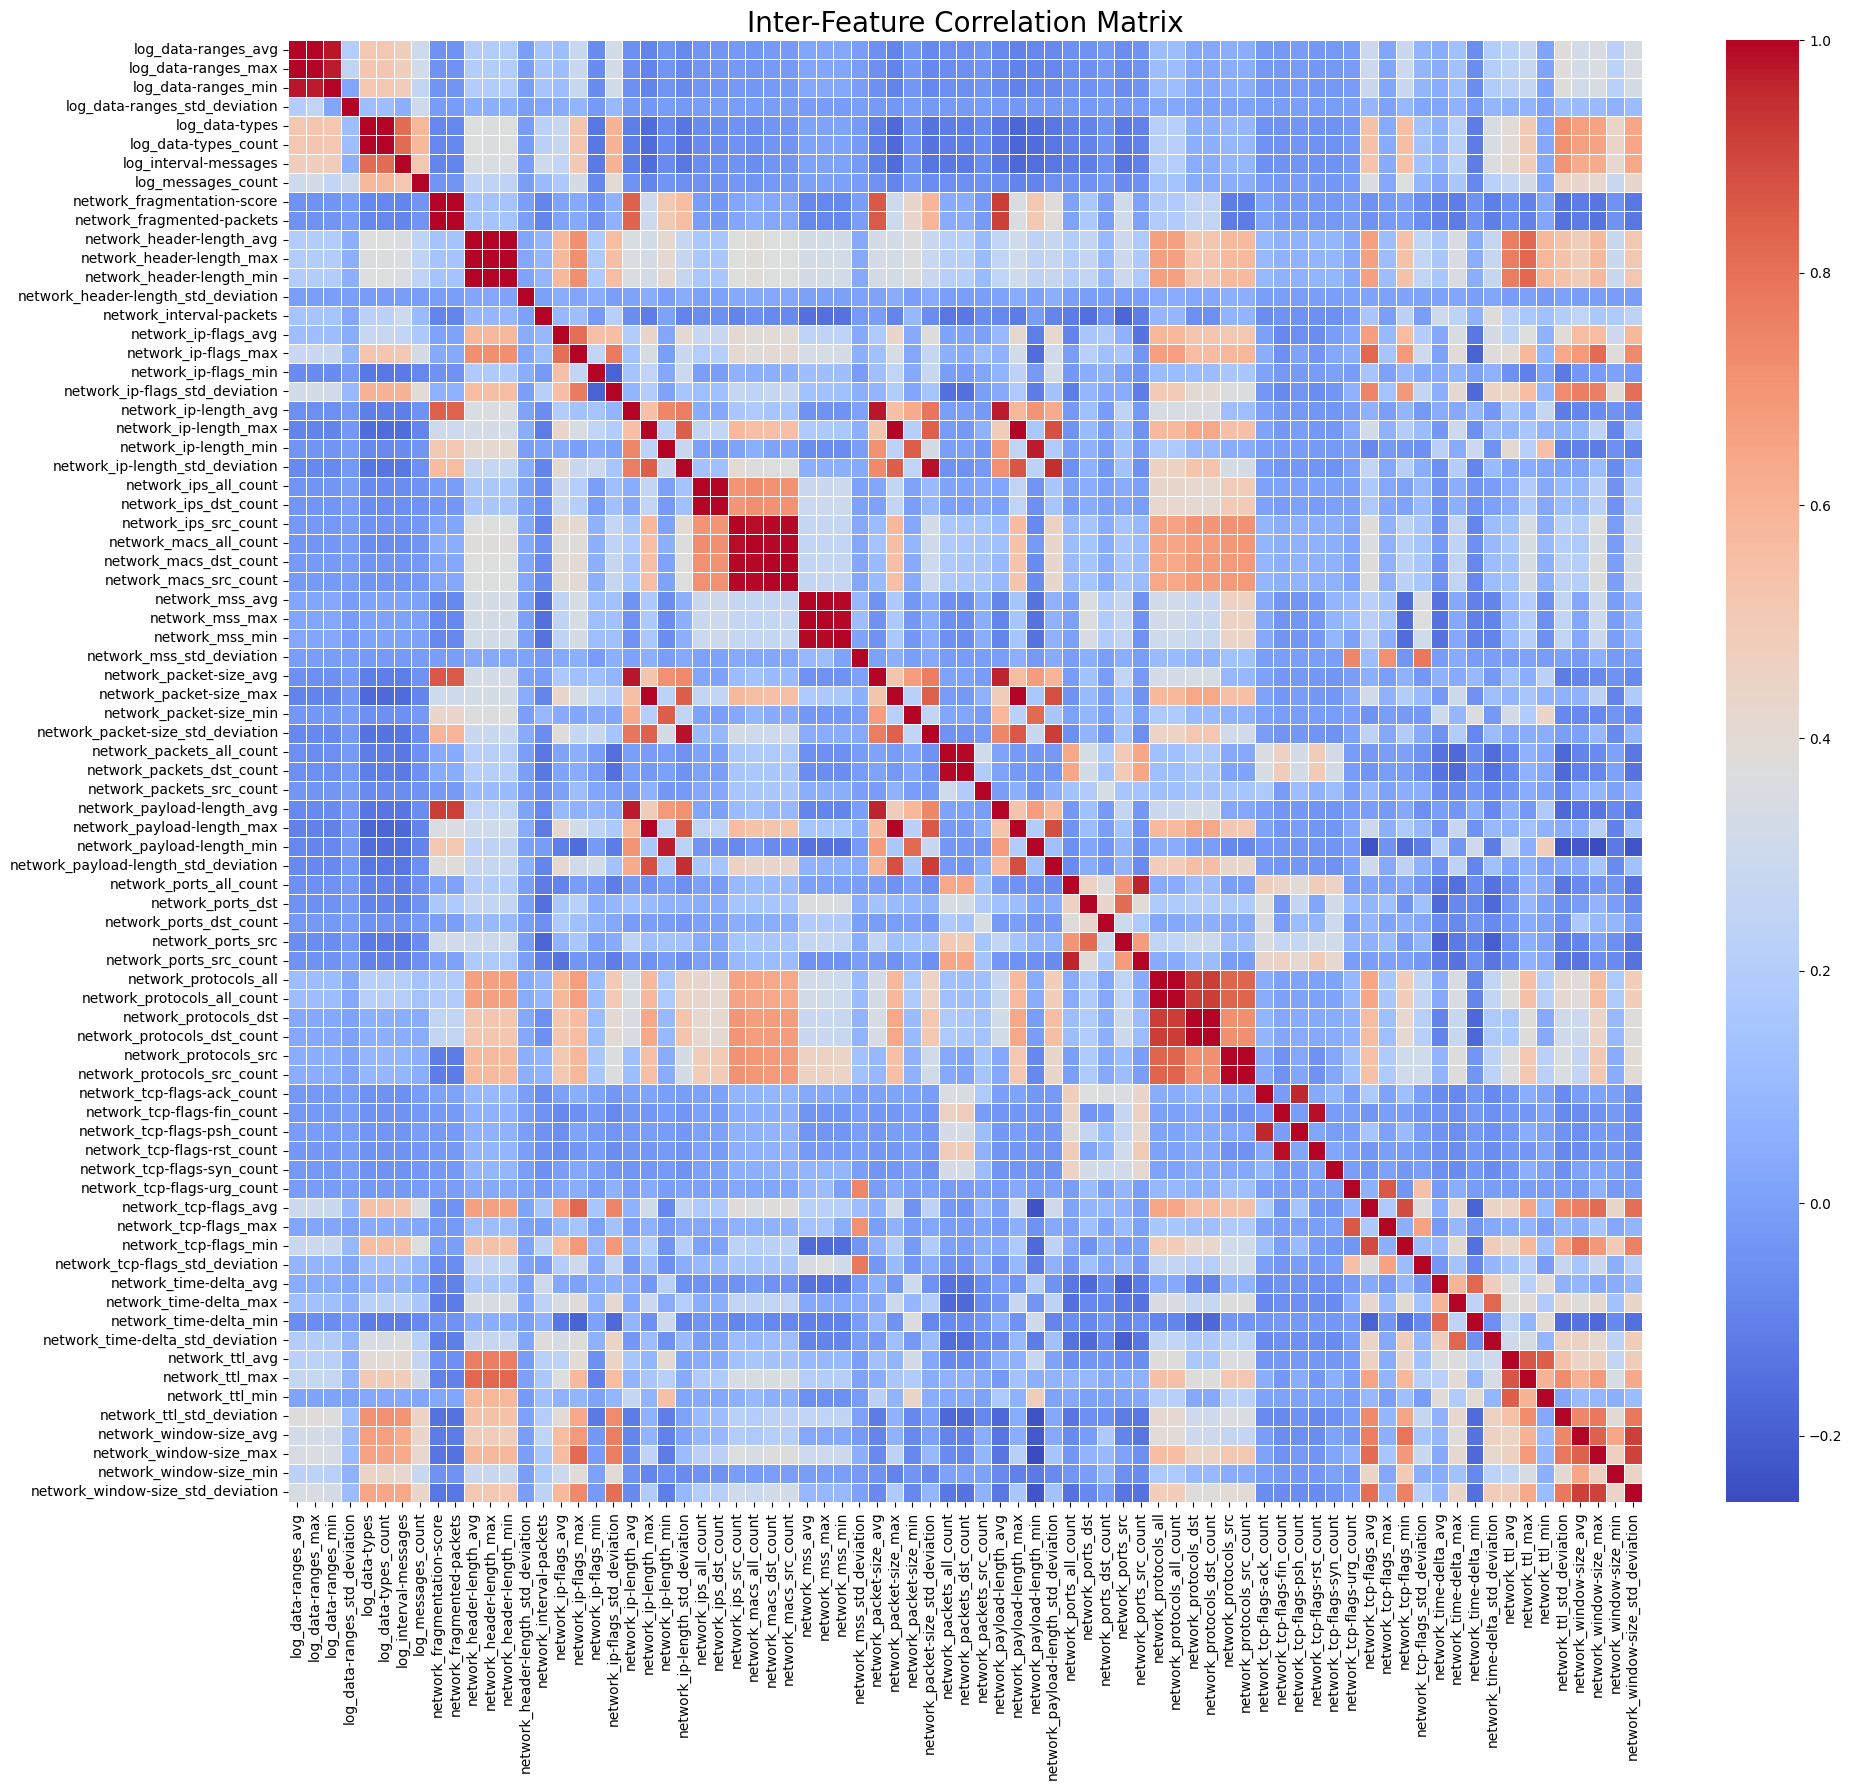
\includegraphics[width=5in]{Images/correlation_heatmap.png}}
			{\rule{5in}{4in} % Placeholder -- add file at Images/correlation_heatmap.png
			\\[-4.2cm]\centering\textit{\small [Image not yet added: Images/correlation\_heatmap.png]}\\[4in]}
	\end{center}
	\caption{Pairwise correlation heatmap of the 81-feature dataset used to identify the 25 features removed in Step 3 of the preprocessing pipeline (correlation $>0.95$ with another retained feature).}
	\label{fig:correlation_heatmap}
\end{figure}

\FloatBarrier
\section{Cloud Layer: Threat Classification and XAI}\label{sec:cloud_classification}

The edge gateway forwards every completed traffic window to the cloud tier over the \textbf{Cloud-Edge Communication} channel shown in Figure \ref{fig:architecture}, via a single HTTP ingestion endpoint that accepts the window's raw, per-connection records (device identifier, window start/end timestamps, and the list of individual connection-log entries observed in that window) rather than a pre-computed feature vector or risk score. This channel is deliberately bidirectional and is drawn as a distinct component in the architecture rather than folded into either tier, because it carries two structurally different kinds of traffic that must both be accommodated without contending with the gateway's normal operational load: raw windowed telemetry flows upward from the edge gateway to the cloud tier's classification pipeline, while \textit{Commands \& Healing Actions} flow downward from the healing-decision pipeline back to the edge gateway. As noted in Section \ref{sec:hybrid_ensemble}, this upward flow is independent of the edge's own risk score; the cloud performs its own classification on every window it receives.

\textbf{Feature construction.} A feature-builder module converts the list of raw connection records in a window into a fixed-length numeric vector matching the schema the classifier was trained on. This schema was derived offline through a four-stage preprocessing pipeline applied to the CIC IIoT 2025 dataset (also released as DataSense), a real-time sensor-and-network-traffic benchmark developed by the Canadian Institute for Cybersecurity from a 40-device industrial testbed spanning more than 15 sensor types, released in December 2024 \cite{Firouzi2025}. The dataset's native representation begins at 94 columns per two-second aggregation window (47 numerical, 24 count-based, and 23 object-type or identifier columns); Step 1 removes device-specific identifiers and overlapping multi-level label columns (94 $\to$ 88 features); Step 2 removes raw address-list object-type columns (full IP- and MAC-address lists) that are unique to the collection testbed and would otherwise let a classifier memorise specific devices rather than learn transferable attack patterns, retaining only their associated count-based features (88 $\to$ 81); Step 3 removes 25 features found to be pairwise-correlated above 0.95 with another retained feature (81 $\to$ 53), eliminating redundant signal rather than distinct information (Figure \ref{fig:correlation_heatmap}); and Step 4 fits an XGBoost classifier on the resulting 53-feature, 112{,}117-record cleaned dataset and retains only the top 30 features by gain-based importance, a 43\% reduction from 53 (Figure \ref{fig:feature_importance})-this final 30-feature set is the schema the deployed classifier described in this section expects. Because the edge layer forwards connection-log-style aggregates-per-connection byte and packet counts, connection state, ports, protocol-rather than true packet-level captures, only a subset of this 30-feature schema can be populated from genuinely observed data at inference time; features that depend on packet-level signals unavailable at this granularity (for example, IP time-to-live statistics, TCP window size, and maximum-segment-size) are populated with a fixed placeholder value rather than left undefined, so that the vector remains well-formed but is not fully informative on every dimension. This gap between the granularity the classifier was trained on and the granularity the edge layer can practically supply is, as discussed in Chapter \ref{cha:results}, the single most consequential limitation identified when this pipeline was evaluated end-to-end.

\begin{figure}[htbp]
	\begin{center}
		\IfFileExists{Images/feature_importance.png}
			{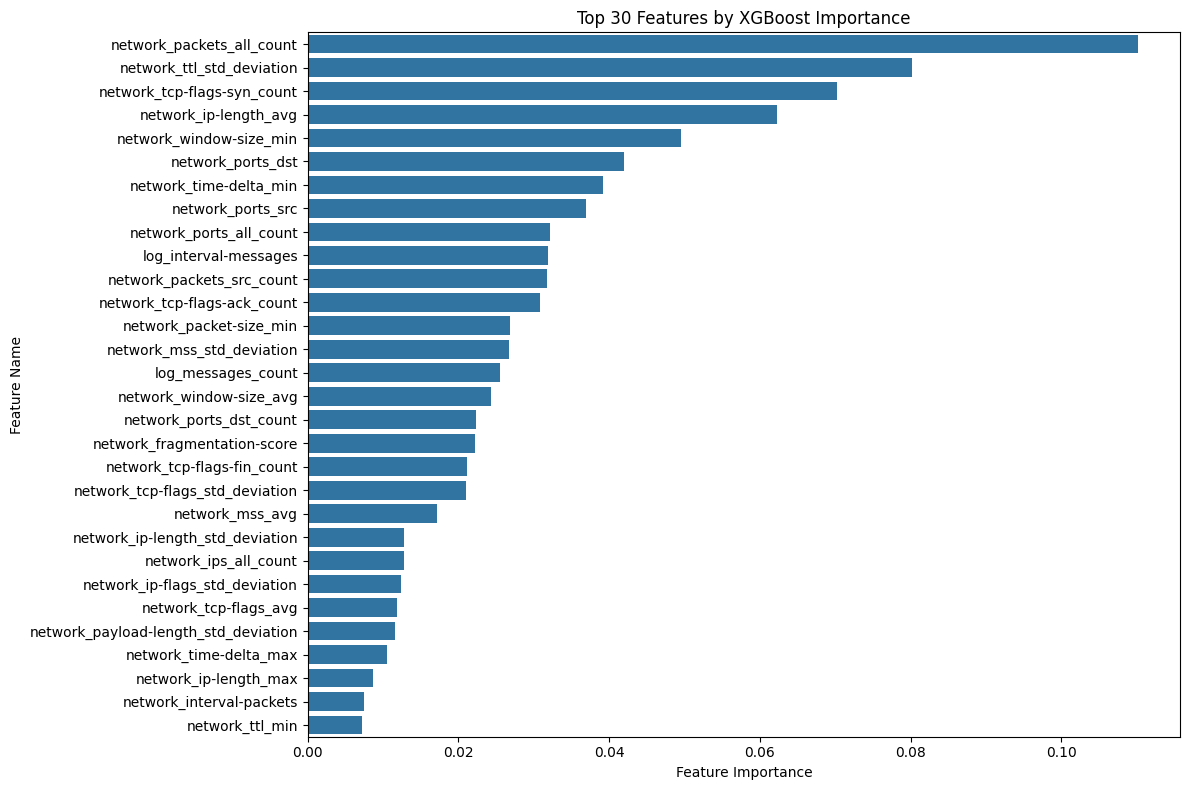
\includegraphics[width=5in]{Images/feature_importance.png}}
			{\rule{5in}{4in} % Placeholder -- add file at Images/feature_importance.png
			\\[-4.2cm]\centering\textit{\small [Image not yet added: Images/feature\_importance.png]}\\[4in]}
	\end{center}
	\caption{Gain-based feature importance ranking from the XGBoost model fitted in Step 4 of the preprocessing pipeline, used to select the top 30 of the remaining 53 features.}
	\label{fig:feature_importance}
\end{figure}

\textbf{Classification.} In the cloud, a pre-trained XGBoost classifier categorizes the specific attack type from the constructed feature vector. XGBoost \cite{ChenGuestrin2016} is a gradient-boosted decision-tree ensemble that builds an additive sequence of shallow regression trees $\hat{y} = \sum_{k=1}^{K} f_k(x)$, where each tree $f_k$ is fitted to reduce the residual error left by the trees before it, subject to an explicit regularization penalty on tree complexity that discourages overfitting to any single training batch of attack traffic. It is selected for this stage over a comparable neural classifier because, on the tabular, engineered flow-features produced by the edge layer's windowing step, tree-boosting ensembles of this kind have consistently matched or exceeded deep-learning classifiers in both accuracy and inference speed on network-flow benchmarks, as discussed in the literature reviewed in Chapter \ref{cha:literature_review}, while remaining directly compatible with the feature-attribution method described next.

The classifier is trained against a fine-grained label set considerably larger than the set of remediation playbooks documented in Appendix \ref{app:healing_actions}: dozens of specific attack sub-types (for example, distinct fine-grained labels for different DDoS flood variants, or for SSH- versus Telnet-targeted brute-force) rather than one label per attack class. Rather than requiring a separate healing playbook for every fine-grained label, the classifier's predicted class probabilities are summed into a small number of \textit{grouped buckets}-\texttt{benign}, \texttt{ddos}, \texttt{port\_scan}, \texttt{bruteforce}, \texttt{mirai\_botnet}, \texttt{lateral\_movement}, \texttt{exfiltration}, and a catch-all \texttt{unhandled\_attack} bucket for fine-grained labels (such as man-in-the-middle and web-application labels) that do not map onto any of the other seven-and the winning bucket's summed probability becomes the reported classification confidence. Both the fine-grained label and the grouped bucket are retained: the grouped bucket is what the healing ladder in Section \ref{sec:multi_agent} keys its playbook selection on, while the fine-grained label is what the SHAP explainer below explains against and what appears in every downstream forensic report. Two of the eight grouped buckets, \texttt{lateral\_movement} and \texttt{exfiltration}, are configured with their own healing playbooks in Appendix \ref{app:healing_actions} but, as verified during evaluation (Chapter \ref{cha:results}), are not currently reachable in practice: no fine-grained label the classifier can output maps onto either bucket, so these two playbooks exist as configured policy without a corresponding trigger path. The training data underlying the feature schema described above (Section \ref{sec:hybrid_ensemble}) itself documents 50 distinct attack types across seven categories-DDoS, DoS, Reconnaissance, Web, Bruteforce, MITM, and Malware/Mirai \cite{Firouzi2025}-and neither \texttt{lateral\_movement} nor \texttt{exfiltration} corresponds to a category in that taxonomy, which is consistent with, and a plausible explanation for, why the classifier has no path to either bucket. The deployed classifier's 76-label fine-grained set does not map one-to-one onto this 50-type source taxonomy, and confirming the exact relationship between the two-whether the production label set extends this dataset's categories with additional sub-types, or was assembled from a broader combination of sources-is noted as a further open item alongside the other integration gaps discussed in Section \ref{sec:limitations_integration}.

A classification is only acted upon by the healing pipeline once its confidence exceeds a fixed gate; classifications below the gate do not open an incident on their own, but are tracked as a rolling low-confidence signal for the same device and attack-type pairing, as described in Section \ref{sec:multi_agent}.

\textbf{Explainability.} Crucially, the classification is passed through a SHAP explainer, computed against the predicted \textit{fine-grained} label rather than the grouped bucket, so that the explanation reflects exactly which sub-type of attack the model believes it has seen. SHapley Additive exPlanations (SHAP), introduced by Lundberg and Lee \cite{Lundberg2017}, assigns each input feature $i$ a contribution value
\begin{equation}
\phi_i = \sum_{S \subseteq F \setminus \{i\}} \frac{|S|!\,(|F|-|S|-1)!}{|F|!} \Big[ f(S \cup \{i\}) - f(S) \Big],
\label{e:shap}
\end{equation}
where $F$ is the full set of input features, $S$ ranges over every subset of the other features, and $f(S)$ is the classifier's expected output when only the features in $S$ are known. Equation \ref{e:shap} is the Shapley value from cooperative game theory, applied here by treating each network feature as a ``player'' contributing to the classifier's output; it has the property that the contributions $\phi_i$ sum exactly to the difference between the model's prediction for a given window and its average prediction, so the attribution is additive and exact rather than a heuristic approximation. Only the top-3 contributing features by $|\phi_i|$ are retained, each tagged with the direction of its contribution, and translated from raw feature codes into short plain-English statements before being passed downstream (for example, describing a high count of unanswered SYN packets as evidence pushing the classification toward a particular attack class). Instead of presenting this XAI output solely to human administrators, the translated SHAP attributions and classification labels are serialized and fed directly into the cognitive healing pipeline described next.

\textbf{Attribution faithfulness.} Because the downstream healing pipeline consumes SHAP attributions directly rather than as an advisory overlay, the attributions themselves must be verified to reflect features the classifier actually relies on rather than plausible-looking but incidental ones. This is quantified with the standard \textit{correctness deletion curve}: features are removed in descending order of $|\phi_i|$ and, at each step, the classifier's average probability assigned to the originally predicted (true) class is measured on the remaining perturbed vector, tracing how quickly the model's confidence collapses as its own top-attributed features are withdrawn. Figure \ref{fig:correctness_deletion} shows the resulting curve on the held-out evaluation set: the true-class probability falls from 0.89 with all features present to 0.50 after removing only the top $\sim$3\% of features, and to 0.22 after removing the top $\sim$7\%, before flattening near the class-prior baseline once roughly 40\% of features have been withdrawn. The area under this perturbation curve (AUPC) is 0.1264, and the sharp, front-loaded drop directly supports the interpretation that the features SHAP surfaces are the ones the classifier is genuinely acting on; the top-3 statements passed to the healing pipeline can therefore be treated as decision-driving evidence rather than post-hoc rationalisation.

\begin{figure}[htbp]
	\begin{center}
		\IfFileExists{Images/correctness_deletion_curve.jpeg}
			{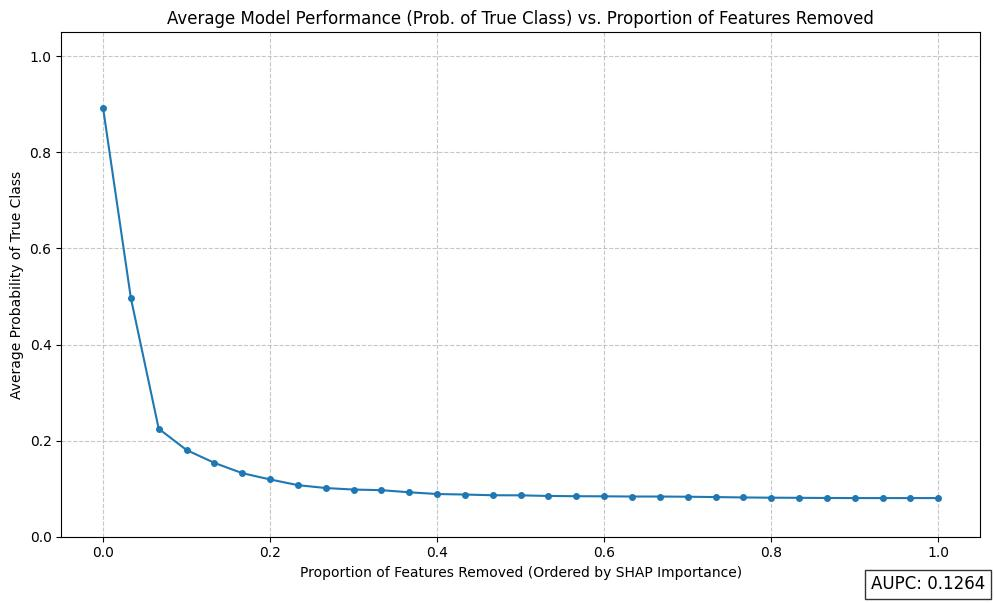
\includegraphics[width=5in]{Images/correctness_deletion_curve.jpeg}}
			{\rule{5in}{3in} % Placeholder -- add file at Images/correctness_deletion_curve.jpeg
			\\[-3.2cm]\centering\textit{\small [Image not yet added: Images/correctness\_deletion\_curve.jpeg]}\\[3in]}
	\end{center}
	\caption{Correctness deletion curve for the SHAP attributions produced by the cloud-tier XGBoost classifier: average probability of the originally predicted (true) class as a growing proportion of features, ordered by descending SHAP importance, is withheld from the input. The steep front-loaded drop (AUPC = 0.1264) indicates that the top-attributed features are the ones the classifier is genuinely acting on.}
	\label{fig:correctness_deletion}
\end{figure}

\FloatBarrier

\section{Multi-Agent System and Self-Healing Orchestration}\label{sec:multi_agent}

Unlike an architecture in which every classified window is handed to a language model to decide a response, the cognitive core of this framework treats the language model as a \textit{fallback} mechanism rather than the default decision-maker. The primary healing decision is made by a deterministic \textbf{ladder engine} operating over the prioritised playbooks documented in Appendix \ref{app:healing_actions}; a language-model agent is only consulted when that deterministic mechanism cannot make a confident decision on its own. This design choice follows directly from the explainability argument developed in Chapter \ref{cha:literature_review}: a playbook whose escalation order is fixed in advance and auditable in a table is inherently more inspectable, before the fact, than a decision an LLM generates fresh each time, so the deterministic path is preferred whenever it is applicable and the language model is reserved for the cases the playbook genuinely cannot cover.

Three distinct roles are served by language-model agents in this design, rather than a single sequential pipeline:

\begin{enumerate}
	\item \textbf{Dashboard Reporting Agent:} Runs on every classification the cloud tier produces, independently of and in parallel with the healing decision described below-a report is generated whether or not any healing action is taken, so that an operator watching the dashboard has visibility into benign and sub-threshold windows as well as acted-upon incidents. It synthesizes the classification, the translated SHAP attributions, and the raw window's descriptive statistics into a structured, human-readable security report (a summary, a severity rating, and a set of indicators), either through a language-model call or, in constrained deployments, a deterministic template.
	\item \textbf{Decision Agent (LLM Fallback):} Consulted only in two specific circumstances the ladder engine cannot resolve on its own: a classification whose confidence stays below the confidence gate on repeated occasions for the same device and attack-type pairing (a persistent low-confidence streak, rather than a single uncertain window), or a classification that lands in the \texttt{unhandled\_attack} bucket, for which no ladder is configured at all (Section \ref{sec:cloud_classification}). In either case, the Decision Agent is grounded by the same Retrieval-Augmented Generation (RAG) mechanism described below and chooses a single action from the healing catalogue, rather than free-composing an arbitrary command.
	\item \textbf{Escalation Agent (Human-Handoff Reporting):} Consulted only once an incident reaches the final tier of its playbook without the device's risk resolving, or once a Decision Agent-selected action itself proves ineffective. Rather than choosing a further automated action, this agent's sole output is a structured operator brief-a plain-language account of the incident timeline and everything already attempted-attached to the incident at the moment it is handed to a human, matching the escalation behaviour already described qualitatively in Chapter \ref{cha:introduction}.
\end{enumerate}

The RAG mechanism that grounds the Decision and Escalation Agents follows the general retrieval-augmented generation pattern introduced by Lewis et al. \cite{Lewis2020}: the markdown-formatted playbooks of Appendix \ref{app:healing_actions}, together with hardware, topology, and policy documents describing the specific edge deployment, are embedded into a vector representation and indexed in advance, and at query time an agent's request (informed by the classification and the translated SHAP attributions) is embedded in the same space and matched against the index to retrieve only the passages most relevant to the device and incident at hand. This retrieved context is then inserted into the prompt given to the language model, so that its output is conditioned on verified, deployment-specific facts-for instance, which VLANs actually exist on the affected switch-rather than on statistically plausible but potentially incorrect assumptions about the network's configuration. A successful Decision Agent action is, in turn, written back into this same retrieval corpus once its effectiveness is confirmed (see \textit{Healing Actions and Closed-Loop Feedback} below), so that the knowledge base a future incident is grounded against includes not only the static playbooks but a growing record of what has actually worked.

\begin{figure}[htbp]
	\begin{center}
	\resizebox{5.5in}{!}{%
	\begin{tikzpicture}[
		>=Stealth,
		node distance=0.65cm,
		data/.style={draw=blue!80, fill=blue!5, rectangle, rounded corners, minimum height=0.7cm, text centered, text width=4.6cm, font=\scriptsize},
		report/.style={draw=teal!80, fill=teal!5, rectangle, rounded corners, minimum height=0.7cm, text centered, text width=3.0cm, font=\scriptsize},
		ladder/.style={draw=purple!80, fill=purple!5, rectangle, rounded corners, minimum height=0.7cm, text centered, text width=3.6cm, font=\scriptsize},
		agent/.style={draw=orange!80, fill=orange!5, rectangle, rounded corners, minimum height=0.7cm, text centered, text width=3.6cm, font=\scriptsize},
		rag/.style={draw=gray!80, fill=gray!10, cylinder, shape border rotate=90, aspect=0.22, minimum height=1.3cm, text centered, text width=2.1cm, font=\scriptsize},
		decision/.style={draw=red!80, fill=red!5, diamond, aspect=2.6, inner sep=1pt, text centered, text width=2.5cm, font=\scriptsize},
		outcome/.style={draw, rectangle, rounded corners, minimum height=0.65cm, text centered, text width=2.4cm, font=\scriptsize},
		arrow/.style={->, thick}
	]

	\node[data] (env) {Classified envelope\\ (label, fine\_label, confidence, SHAP)};

	\node[report, right=1.4cm of env] (reporter) {Dashboard Reporting Agent\\ (every window, parallel)};

	\node[decision, below=0.6cm of env] (benign) {Benign?};
	\node[decision, below=0.6cm of benign] (gate) {Confidence $\geq$ gate,\\ or streak met?};
	\node[decision, below=0.75cm of gate] (haslad) {Ladder exists\\ for bucket?};

	\node[outcome, left=1.3cm of benign, fill=green!8, draw=green!70] (nostreak) {Increment streak;\\ no incident};
	\node[outcome, left=1.3cm of gate, fill=gray!8, draw=gray!60] (wait) {Wait\\ (no action\\ this window)};

	\node[ladder, below=1.15cm of haslad, xshift=-2.3cm] (laddereng) {Ladder Engine:\\ dispatch level $P_n$};
	\node[agent, below=1.15cm of haslad, xshift=2.3cm] (decagent) {Decision Agent\\ (LLM + RAG)};

	\node[rag, right=1.2cm of decagent] (rag) {\textbf{RAG}\\ Playbooks,\\ hardware,\\ past actions};

	\node[data, below=2.45cm of haslad] (dispatch) {Dispatch via EdgeClient (HTTP)};
	\node[data, below=0.55cm of dispatch] (feedback) {Edge apply / verification feedback};

	\node[decision, below=0.6cm of feedback] (effective) {Effective?};
	\node[decision, below=1.15cm of effective, xshift=-1.8cm] (levels) {Levels\\ remaining?};

	\node[outcome, fill=green!10, draw=green!70, below=1.15cm of effective, xshift=1.8cm] (resolved) {Resolved\\ (decay scheduled)};

	\node[outcome, fill=orange!10, draw=orange!70, below=0.6cm of levels] (approval) {Approval gate\\ (P6 / ESC-02)};
	\node[agent, below=0.55cm of approval] (escagent) {Escalation Agent\\ (LLM + RAG brief)};
	\node[outcome, fill=red!8, draw=red!70, below=0.55cm of escagent] (human) {Human resolves};

	% Arrows: top
	\draw[arrow] (env) -- (reporter);
	\draw[arrow] (env) -- (benign);
	\draw[arrow] (benign.west) -- node[above, font=\tiny] {Yes} (nostreak.east);
	\draw[arrow] (benign) -- node[right, font=\tiny] {No} (gate);
	\draw[arrow] (gate.west) -- node[above, font=\tiny] {No} (wait.east);
	\draw[arrow] (gate) -- node[right, font=\tiny] {Yes} (haslad);

	\coordinate (laddersplit) at ([yshift=-0.45cm]haslad.south);
	\draw[arrow] (haslad.south) -- (laddersplit);
	\draw[arrow] (laddersplit) -| node[pos=0.25, above, font=\tiny] {Yes} (laddereng.north);
	\draw[arrow] (laddersplit) -| node[pos=0.35, above, font=\tiny, align=center] {No: unhandled attack\\ or low-confidence streak} (decagent.north);

	\draw[arrow] (decagent.east) -- node[above, font=\tiny] {Query} ([yshift=4pt]rag.west);
	\draw[arrow] ([yshift=-4pt]rag.west) -- node[below, font=\tiny] {Context} (decagent.east);

	\draw[arrow] (laddereng.south) -- ++(0,-0.3cm) -| ([xshift=-1.1cm]dispatch.north);
	\draw[arrow] (decagent.south) -- ++(0,-0.3cm) -| ([xshift=1.1cm]dispatch.north);
	\draw[arrow] (dispatch) -- (feedback);
	\draw[arrow] (feedback) -- (effective);

	\coordinate (effectivesplit) at ([yshift=-0.4cm]effective.south);
	\draw[arrow] (effective.south) -- (effectivesplit);
	\draw[arrow] (effectivesplit) -| node[pos=0.25, above, font=\tiny] {No} (levels.north);
	\draw[arrow] (effectivesplit) -| node[pos=0.25, above, font=\tiny] {Yes} (resolved.north);
	\draw[arrow] (levels.west) -- ++(-1.1cm,0) |- node[pos=0.25, left, font=\tiny, align=right] {Yes: escalate\\ to next level} (laddereng.west);
	\draw[arrow] (levels.south) -- node[right, font=\tiny] {No: P6 exhausted} (approval);
	\draw[arrow] (approval) -- (escagent);
	\draw[arrow] (escagent) -- (human);

	\coordinate (join) at ([yshift=-0.5cm]human.south);
	\coordinate (rightlane) at ([xshift=0.9cm]rag.east);
	\draw[gray!55] (resolved.south) |- (join);
	\draw[gray!55] (human.south) |- (join);
	\draw[arrow, gray!55, dashed] (join) -| (rightlane) -- (rag.east);
	\node[rotate=90, font=\tiny, text=gray!55, anchor=south] at ([yshift=-1.2cm]rightlane) {Log outcome as past action};

	\end{tikzpicture}%
	}
	\end{center}
	\caption{Flowchart of the healing decision pipeline: a deterministic ladder engine is the primary path for any classification that crosses the confidence gate and maps to a configured playbook; the Decision Agent (LLM + RAG) is consulted only for the \texttt{unhandled\_attack} bucket or a sustained low-confidence streak, and the Escalation Agent (LLM + RAG) is consulted only once a ladder is exhausted or an LLM-selected action proves ineffective. The Dashboard Reporting Agent runs independently of this decision path on every classified window. Both terminal outcomes write their result back into the RAG knowledge base as a past action.}
	\label{fig:multiagent}
\end{figure}

\textbf{Healing Actions and Closed-Loop Feedback.} Once the Ladder Engine or Decision Agent selects an action, it is dispatched to the edge layer by a single code path (\texttt{EdgeClient}) as an HTTP request to a fixed healing-actions endpoint on the edge gateway; a \textit{dry-run} configuration flag allows every command to be built, logged, and shown on the operator dashboard without actually being delivered, which is the mode used during the verification testing reported in Chapter \ref{cha:results}. Figure \ref{fig:architecture} identifies four categories of action available at the \textbf{Edge Enforcement \& Mitigation} module: \textit{VLAN isolation}, which moves a compromised or suspect device into a restricted broadcast domain that limits which other hosts it can reach; \textit{bandwidth allocation}, which throttles the network capacity available to a specific device or port, directly limiting the volume of traffic-malicious or otherwise-it can generate; \textit{port blocking}, which disables a specific switch or device port outright; and \textit{local response actions}, a fallback category of gateway-local mitigations that do not require a network-wide reconfiguration, such as rate-limiting a single device's traffic locally at the gateway or flagging the device for manual inspection. Every dispatched command resolves to one or more atomic actions from the shared catalogue in Appendix \ref{app:healing_actions}, each of which falls into exactly one of these four categories.

The edge layer reports back on a dispatched command in one of two phases, and these are the only two evidence sources this framework has for ``did the action work'': an \textit{apply} report, confirming whether the command was actually enacted on the device (\texttt{applied}, \texttt{skipped}, \texttt{unsupported}, or \texttt{failed}), and a \textit{verification} report, sampled after a short delay, confirming whether the action actually resolved the condition it was dispatched for (\texttt{effective: true/false}). An apply failure short-circuits directly to the escalation decision without waiting for verification; where both signals are available, verification is authoritative. Separately, if the same device and attack-type classification recurs while an incident is already open, that recurrence is itself treated as evidence that the incident is still active, independently of whatever the edge reports.

If verification confirms the action was effective, the incident is marked resolved and, if it had escalated above the first level, a decay is scheduled so that any standing mitigation is relaxed once the hold period elapses-mirroring, at the remediation layer, the same decay behaviour the edge-side risk score exhibits in Equation \ref{e:risk_decay}. If verification reports the action was not effective (or the apply itself failed), the incident advances to the next tier of the same playbook rather than repeating the tier that already failed; if no further tier exists, the incident is parked at an approval gate and handed to the Escalation Agent for a human-readable operator brief, matching the escalation behaviour already described qualitatively in Chapter \ref{cha:introduction}. In either terminal case, the outcome-which action was taken, against which classification, and whether it worked-is written back into the RAG knowledge base's retrieval corpus as a past action, so that a Decision Agent facing a similar incident in future has access to a growing record of what has actually worked, not only the static playbook definitions.

\textbf{Prioritised Escalation Playbooks.} The four action categories in Figure \ref{fig:architecture} are deliberately abstract because each one is, in practice, backed by a structured, per-attack-class playbook rather than a single flat command. For every grouped bucket the cloud-tier classifier can output and for which a playbook is configured, the Ladder Engine holds an ordered sequence of priority tiers running from the least disruptive action to the most disruptive, so that the escalation path in Figure \ref{fig:multiagent} has a concrete ladder to climb rather than an unstructured set of options to choose between arbitrarily. For a classified DDoS attack, for instance, the first tier applies stateless rate limiting and flood-specific hardening at the gateway (enabling SYN cookies and capping half-open connections, without dropping any legitimate session); only if verification reports the action ineffective does the engine advance to blocking the highest-contributing sources, then to prefix-level aggregate blocking and uplink shaping, then to moving the device into a quarantine VLAN, then to a graceful reboot or power cycle, and finally, if none of the preceding tiers succeeds, to full isolation and escalation to a human operator. Every tier in every such playbook resolves to one or more atomic actions from the shared catalogue (for example, \texttt{NET-01} for adaptive rate limiting or \texttt{SEG-01} for quarantine VLAN assignment), and a small set of observation actions (packet capture, sensitivity boosting) run in parallel with the priority ladder rather than as a step within it, so that forensic evidence is preserved regardless of which remediation tier is ultimately reached. The benign case is handled by the same mechanism in reverse: as a device's classification returns to benign and any open incident's mitigation decay timer elapses, standing mitigations are relaxed in step-TTL-based blocks expire, rate limits lift, and a quarantined device is returned to its normal VLAN-so that a device is not left restricted indefinitely once the threat that triggered the restriction has genuinely passed, mirroring the edge-side risk-decay behaviour of Equation \ref{e:risk_decay}. As noted in Section \ref{sec:cloud_classification}, two of the eight grouped buckets (\texttt{lateral\_movement} and \texttt{exfiltration}) have a configured playbook in Appendix \ref{app:healing_actions} but no classifier path that currently reaches it; this is discussed further as a limitation in Chapter \ref{cha:results}. The full catalogue of atomic actions and the complete prioritised playbook for every reachable attack class this framework classifies are documented in Appendix \ref{app:healing_actions}.

\section{Communication and Transport-Layer Security}\label{sec:comm_security}

The healing pipeline described in Sections \ref{sec:cloud_classification} and \ref{sec:multi_agent} depends on two communication boundaries that must themselves be trustworthy before any telemetry, classification, or healing command is allowed to cross them: the link between an IoT device and its edge hub, and the link between the hub and the layer that surfaces its activity outward. Both boundaries are secured by mechanisms independent of, and prior to, the detection and remediation logic itself.

\subsection{Device to Hub (Edge): Two-Stage Mutual Authentication and Encrypted Telemetry}

Before any telemetry is accepted from a device, the hub validates that device through a two-stage handshake. In the first stage, every device is pre-provisioned by a dedicated provisioning script, which generates a 2048-bit RSA keypair, stores the private key on the device itself, and registers the corresponding public key in a shared device registry; each registry entry is signed by a 3072-bit root Certificate Authority (CA) key so that the registry itself cannot be tampered with undetected. When a device connects, the hub first looks up the registry and verifies that the device's public-key entry carries a valid root CA signature-a chain-of-trust check that rejects any device whose registry entry was not signed by the deployment's own root key. The hub then issues a 32-byte random nonce as a challenge; the device signs this nonce with its RSA private key using PKCS\#1~v1.5 padding over SHA-256, and the hub verifies the resulting signature against the device's registered public key. This proves the device possesses the private key corresponding to its registered identity without the private key ever being transmitted. Only once this proof-of-possession succeeds does the hub generate a fresh 256-bit AES session key, encrypt it under the device's RSA public key using PKCS\#1-OAEP padding, and return it to the device, ensuring that only the device which just proved its identity can unwrap the session key.

The second stage governs the telemetry itself. Every subsequent packet is encrypted with AES-256 in CBC mode under a random initialisation vector generated per packet, so that no two packets, even with identical plaintext, produce the same ciphertext. Each packet additionally carries a SHA-256 integrity hash, a UTC timestamp that the hub rejects if its drift from the hub's own clock exceeds five seconds, and a strictly monotonic per-device counter; together, these three fields defend against replay attacks, out-of-order packet injection, and in-flight tampering, independently of the confidentiality provided by the AES encryption itself. At the transport level, the hub additionally enforces per-source-IP rate limiting (a maximum of 40 connection attempts per 60-second window) and issues temporary IP bans on repeated authentication failures, mitigating brute-force key-guessing and connection-exhaustion denial-of-service attempts against the handshake itself.

\subsection{Hub to Cloud (Dashboard) Communication}

In this architecture, the ``cloud'' boundary is the hub's own read-only HTTP dashboard endpoint (\texttt{/api/events}), which serves a JSON event log of activity across both handshake stages described above. Access to this boundary is deliberately narrow: it exposes only a single \texttt{GET} endpoint, every response is sent with a \texttt{Cache-Control: no-store} header so that event data is never retained in an intermediate cache, and all event data is HTML-escaped before rendering to prevent cross-site scripting (XSS) against any client viewing the dashboard. The hub never forwards raw device credentials, private keys, or session keys to this layer; only sanitised, already-decrypted telemetry summaries and audit events are surfaced outward, so that a compromise of the dashboard boundary cannot, by itself, expose the material needed to impersonate a device or decrypt its traffic.

\section{Time Plan and Resources Required}

\textbf{Time Plan.} Table \ref{tb:timeline} sets out the week-by-week schedule (rotated to landscape given its width) followed across the eight-month project timeline, from problem definition through to final documentation and dissemination. Progress is tracked at milestone granularity rather than by individual task, with each milestone spanning the number of weeks shown as shaded in the corresponding row; the three-stage implementation structure (edge node, ML detection and healing, then XAI and LLM-based adaptive reasoning) is deliberately sequential, with each stage's completion gating the start of the next, before the three stages are brought together in the integration and closed-loop learning milestone that precedes the evaluation phase (known-attack simulation, zero-day and stress testing, and comparative benchmarking) and the final write-up.

\newcommand{\Y}{\cellcolor{gray!70}}
\begin{sidewaystable}
\centering
\caption{Project timeline and progress by week (shaded cells indicate the completed period for each milestone).}
\label{tb:timeline}
\renewcommand{\arraystretch}{1.3}
\setlength{\tabcolsep}{2pt}
\footnotesize
\begin{tabular}{|p{4.5cm}|*{30}{c|}}
\hline
\textbf{Month} & \multicolumn{4}{c|}{Jan} & \multicolumn{4}{c|}{Feb} & \multicolumn{5}{c|}{Mar}
& \multicolumn{3}{c|}{Apr} & \multicolumn{4}{c|}{May} & \multicolumn{4}{c|}{Jun}
& \multicolumn{3}{c|}{Jul} & \multicolumn{3}{c|}{Aug} \\
\hline
\textbf{Milestone} &
1&2&3&4&5&6&7&8&9&10&11&12&13&14&15&16&17&18&19&20&21&22&23&24&25&26&27&28&29&30 \\
\hline
Problem Definition \& Literature Review Completed -- Research objectives, threat model, evaluation metrics, and dataset plan finalized. &
\Y&\Y&\Y&\Y& & & & & & & & & & & & & & & & & & & & & & & & & & \\
\hline
System Architecture \& Testbed Design Finalized &
& & & &\Y&\Y&\Y& & & & & & & & & & & & & & & & & & & & & & & \\
\hline
Stage 1 Edge Node Implementation Completed &
& & & & & & &\Y&\Y&\Y& & & & & & & & & & & & & & & & & & & & \\
\hline
Stage 2 ML Detection \& Healing Implemented &
& & & & & & & & & &\Y&\Y&\Y& & & & & & & & & & & & & & & & & \\
\hline
Stage 3 XAI + LLM Adaptive Reasoning Prototype Ready &
& & & & & & & & & & & & &\Y&\Y&\Y&\Y&\Y& & & & & & & & & & & &\\
\hline
Stage 1--3 Integration \& Closed-Loop Learning Operational &
& & & & & & & & & & & & & & & &  & &\Y&\Y&\Y&\Y& & & & & & & & \\
\hline
Known Attack Simulation Completed &
& & & & & & & & & & & & & & & & & & & & & &\Y&\Y& \Y& & & & & \\
\hline

\hline
Comparative Benchmarking Done &
& & & & & & & & & & & & & & & & & & & & & & & & &\Y& \Y& & & \\
\hline

Final Documentation \& Dissemination &
& & & & & & & & & & & & & & & & & & & & & & & & & & &\Y & &\\
\hline
\end{tabular}
\end{sidewaystable}

\textbf{Resources Required.} Table \ref{tb:budget} itemises the gateway hardware, supporting components, and representative smart-IoT devices required to build and evaluate the prototype. Prices are approximate planning figures in Sri Lankan rupees and should be reconfirmed with local suppliers before procurement. Where no reliable local price was available, the item is marked as to be determined (TBD); consequently, the subtotal reports a range for priced items and excludes the three TBD devices.

{\small
\begin{longtable}{|p{0.48\textwidth}|p{0.14\textwidth}|p{0.28\textwidth}|}
\caption{Project budget and representative IoT-device inventory for the edge-gateway prototype.}
\label{tb:budget}\\
\hline
\textbf{Item} & \textbf{Units} & \textbf{Price (LKR)} \\
\hline
\endfirsthead
\multicolumn{3}{c}{\tablename\ \thetable{} -- continued from previous page}\\
\hline
\textbf{Item} & \textbf{Units} & \textbf{Approx. price (LKR)} \\
\hline
\endhead
\hline \multicolumn{3}{r}{\textit{Continued on next page}}\\
\endfoot
\hline
\endlastfoot
Raspberry Pi 5 & 1 unit & 50{,}400 \\
\hline
Raspberry Pi Zero 2W & 1 unit & 7{,}400 \\
\hline
Cables, wires and AC plugs & 1 lot & 2{,}000 \\
\hline
Enclosure -- Pi 5 & 1 unit & 2{,}250 \\
\hline
Power supply -- Pi 5 & 1 unit & 1{,}100 \\
\hline
Switch & 2 units & 5{,}800 \\
\hline
Wi-Fi Mini Smart Switch & 1 unit & 2{,}390 \\
\hline
Echo Pop (Alexa) & 1 unit & 13{,}300 \\
\hline
Smart Camera & 1 unit & 2{,}800 \\
\hline
Smart Plug & 1 unit & 2{,}790 \\
\hline
Wi-Fi Door/Window Sensor & 1 unit & 2{,}890 \\
\hline
Smart Switch & 1 unit & 2{,}990 \\
\hline
Temperature and Humidity Sensor & 1 unit & 330 \\
\hline
Door/Window Sensor (non-Wi-Fi) & 1 unit & 2{,}000 \\
\hline
Comfast Driver-Free Wireless Adapter & 1 unit & 2{,}800 \\
\hline

\multicolumn{2}{|l|}{\textbf{Priced subtotal }} & \textbf{101{,}240} \\
\hline
\end{longtable}
}

%%%%%%%%%%%%%%%%%%%%%%%%%%%%%%%%%%%%%%%%%%%%%%%%%%%%%%%%%%%%%%%%%%%%%%%%%%%%%%%%%%%%%%%%%%%%%%%%%%
%%%%%%%%%%% END OF FILE
%%%%%%%%%%%%%%%%%%%%%%%%%%%%%%%%%%%%%%%%%%%%%%%%%%%%%%%%%%%%%%%%%%%%%%%%%%%%%%%%%%%%%%%%%%%%%%%%%%